\chapter{Letters}

In the second part we will learn to use various grammatical tools. Even though you may use these less often, I put them before more complex tools like text readers and finders because they are easier to learn and explain. This can create familiarity in a smooth way, and make new students more comfortable.

With a good tool, learning Pāli alphabet can be an enjoyable experience. The Letters window can be opened by selecting menu Grammar > {\faSix \symbol{"F031}} Letters. This tool can show characters of several Pāli scripts, i.e., Devanagari, Khmer, Myanmar, Sinhala, and Thai. The display of all these scripts depends on fonts loaded when the program started, both embedded and external. Figure \ref{fig:letters} shows Pāli letters in Khmer script with some sample input string.

\begin{figure}[!hbt]
\centering
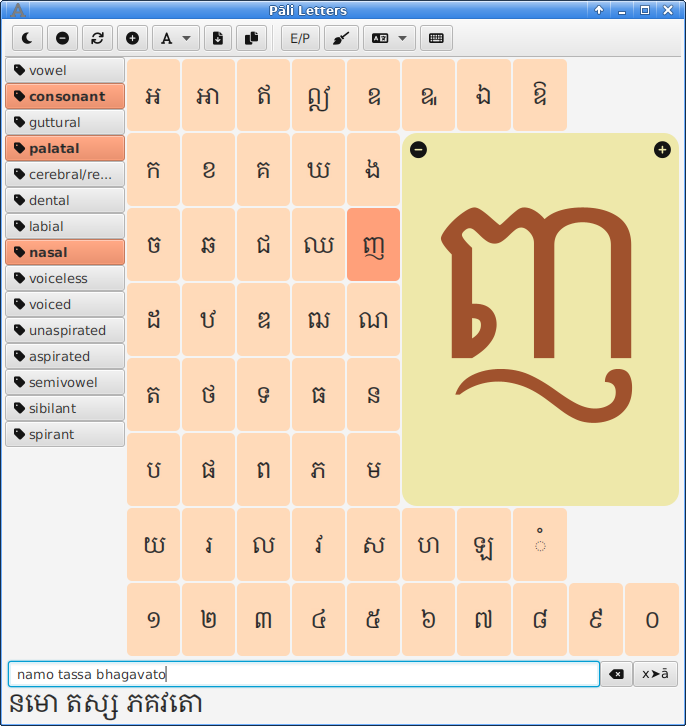
\includegraphics[width=0.9\linewidth]{images/letters.png}\\
\caption{Letters window}
\label{fig:letters}
\end{figure}

As shown in its tool bar, additional buttons are explained below:

\bigskip
\begin{tabular}{ll}
\bfseries \texttt{E/P} & Switch between English and Pāli technical terms\\
{\faSix \symbol{"F51A}} & Clear highlights and selections \\
{\faSix \symbol{"F1AB}} & Select a script language \\
{\faSix \symbol{"F11C}} & Open/close typing test area \\
\end{tabular}
\bigskip

This Letters window is quite obvious to use and enjoyable to learn. So, I will not explain further. It is better to read about Pāli letters first to get the basic idea. For the detail, please learn by doing.
